\documentclass[12pt,a4paper]{article}
\usepackage[utf8]{inputenc}
\usepackage[T5]{fontenc}
\usepackage[vietnamese]{babel}
\usepackage{geometry}
\usepackage{longtable}
\usepackage{booktabs}
\usepackage{amsmath}
\usepackage[hidelinks,unicode]{hyperref}
\usepackage[table]{xcolor}
\usepackage{lmodern}
\usepackage{enumitem}
\usepackage{caption}
\usepackage{tikz}
\usepackage{graphicx}
\usepackage{indentfirst}
\usepackage{float}
\usepackage{fancyhdr}
\usepackage{titlesec}
\usepackage{tabularx}
\usetikzlibrary{shapes, arrows, positioning, fit, calc, mindmap, trees, shadows}

\geometry{a4paper, margin=1in, top=1.2in}

\pagestyle{fancy}
\fancyhf{}
\fancyhead[L]{\footnotesize Tính toán khoa học thần kinh} % Đổi tiêu đề header trái
\fancyhead[R]{\footnotesize UET - VNU}
\fancyfoot[C]{\thepage}
\renewcommand{\headrulewidth}{0.4pt}
\renewcommand{\footrulewidth}{0.4pt}

% Định dạng section (Giữ nguyên)
\titleformat{\section}
  {\normalfont\Large\bfseries}{\thesection}{1em}{}
\titleformat{\subsection}
  {\normalfont\large\bfseries}{\thesubsection}{1em}{}
\titleformat{\subsubsection}
  {\normalfont\normalsize\bfseries}{\thesubsubsection}{1em}{}

\begin{document}

% =============== TRANG BÌA ===============
\begin{titlepage}
    % --- VẼ KHUNG VIỀN ---
    \begin{tikzpicture}[overlay,remember picture]
        \draw [line width=3pt]
            ($ (current page.north west) + (2.5cm,-2.0cm) $)
            rectangle
            ($ (current page.south east) + (-1.5cm,2.0cm) $);
        \draw [line width=1pt]
            ($ (current page.north west) + (2.65cm,-2.15cm) $)
            rectangle
            ($ (current page.south east) + (-1.65cm,2.15cm) $);
    \end{tikzpicture}

    \centering

    % --- PHẦN 1: HEADER TRƯỜNG & LOGO ---
    \vspace*{0.2cm}
    {\fontsize{14}{16}\selectfont \textbf{ĐẠI HỌC QUỐC GIA HÀ NỘI}}\\[0.2cm]
    {\fontsize{15}{18}\selectfont \textbf{TRƯỜNG ĐẠI HỌC CÔNG NGHỆ}}\\[0.2cm]
    \rule{8cm}{0.8pt}

    \vspace{1.2cm}
    
\includegraphics[width=3.3cm]{uet.png}

    \vspace{1.3cm}

    % --- PHẦN 2: TIÊU ĐỀ ---
    {\fontsize{18}{22}\selectfont \textbf{BÁO CÁO HỌC PHẦN DỰ ÁN}}\\[1.1cm]

    {\fontsize{24}{28}\selectfont \textbf{ĐỀ TÀI}}\\[0.5cm]

    {\fontsize{22}{26}\selectfont
    \textbf{HỆ THỐNG HYBRID - LLM}}\\[0.2cm]
    {\fontsize{22}{26}\selectfont
    \textbf{GIẢI TOÁN KẾT HỢP CHẤM BÀI}}\\[0.2cm]
    {\fontsize{22}{26}\selectfont}

    \vspace{2.4cm}

    % --- PHẦN 3: BẢNG TÊN ---
    \begin{center}
    \large
    \renewcommand{\arraystretch}{1.45}

    \begin{tabular}{l l r}
    \textbf{Giảng viên hướng dẫn:}
    & PGS.TS Nguyễn Việt Hà & \\
    &  ThS. Nguyễn Thị Thùy Linh & \\[0.3cm]

    \textbf{Nhóm sinh viên thực hiện:}
    & Ngô Đình Linh
    & 23020394 \\

    &
    Nguyễn Trần Huy
    & 23020378 \\

    &
    Nguyễn Đức Huy
    & 23020376 \\
    \end{tabular}
    \end{center}

    \vspace{1.0cm}

    % --- PHẦN 4: NGÀY THÁNG ---
    {\large \textbf{Hà Nội, tháng 6 năm 2026}}

\end{titlepage}
% =============== PHẦN CHẤN ĐIỂM VÀ NHẬN XÉT ===============

% =============== Ý KIẾN ĐÁNH GIÁ ===============
\newpage
\thispagestyle{empty}

\begin{center}
    {\Large \textbf{Ý KIẾN ĐÁNH GIÁ}}
\end{center}

\vspace{0.8cm}

\noindent
\textbf{Ý kiến đánh giá:}

\vspace{0.5cm}

\noindent
\makebox[\textwidth]{\dotfill}\\[0.6cm]
\makebox[\textwidth]{\dotfill}\\[0.6cm]
\makebox[\textwidth]{\dotfill}\\[0.6cm]
\makebox[\textwidth]{\dotfill}\\[0.6cm]
\makebox[\textwidth]{\dotfill}\\[0.6cm]
\makebox[\textwidth]{\dotfill}\\[0.6cm]
\makebox[\textwidth]{\dotfill}\\[0.6cm]
\makebox[\textwidth]{\dotfill}\\[0.6cm]
\makebox[\textwidth]{\dotfill}\\[1cm]

\noindent
\textbf{Điểm số:} \dotfill \hspace{1cm}
\textbf{Điểm chữ:} \dotfill

\vspace{1.2cm}

\begin{flushright}
    Hà Nội, ngày \dots, tháng \dots, năm 20\dots
\end{flushright}

\vspace{1cm}

\begin{flushright}
    \textbf{Giảng viên đánh giá}\\
    \textit{(Ký, ghi rõ họ tên)}
\end{flushright}


% =============== LỜI CẢM ƠN ===============
\newpage
\thispagestyle{empty}

\begin{center}
    {\Large \textbf{LỜI CẢM ƠN}}
\end{center}

\vspace{0.8cm}




Lời đầu tiên, chúng em xin được gửi lời cảm ơn chân thành nhất đến thầy Nguyễn Việt Hà và cô Nguyễn Thị Thùy Linh. 
Trong quá trình học tập và thực hiện học phần Dự án, chúng em đã nhận được sự quan tâm, 
hướng dẫn tận tình và những góp ý quý báu từ thầy cô.

Nhờ sự định hướng của cô, nhóm chúng em có thêm cơ hội tìm hiểu, nghiên cứu và triển khai đề tài 
\textbf{``Hệ thống HYBRID-LLM giải toán kết hợp chấm bài''}. 
Đề tài giúp chúng em vận dụng các kiến thức đã học vào việc xây dựng một hệ thống hỗ trợ chấm bài và gia sư học sinh trong quá trình giải toán, 
không chỉ đưa ra đáp án cuối cùng mà còn cung cấp các gợi ý phù hợp nhằm giúp người học hiểu rõ hơn phương pháp giải.

Trong dự án này, nhóm chúng em tập trung xây dựng một hệ thống có khả năng tiếp nhận đề bài hoặc lời giải của học sinh thông qua văn bản hoặc hình ảnh. Đối với dữ liệu hình ảnh, hệ thống sử dụng OCR để trích xuất nội dung bài toán, từ đó hỗ trợ quá trình xử lý đầu vào một cách trực quan và thuận tiện hơn. Bên cạnh đó, nhóm triển khai pipeline gồm các bước \textit{formalize}, \textit{solve} và \textit{verify} cho các bài toán dạng GSM8K. Cụ thể, hệ thống sử dụng mô hình ngôn ngữ lớn để chuyển đổi đề bài và lời giải của học sinh thành các file YAML có cấu trúc, sau đó dùng hàm Python InsideChecker/CompareChecker để kiểm tra các quan hệ tính toán và so sánh lời giải chuẩn với lời giải của học sinh. Trong quá trình thực hiện báo cáo và xây dựng hệ thống, do kiến thức và kinh nghiệm của nhóm còn hạn chế, bài làm chắc chắn khó tránh khỏi những thiếu sót. Chúng em kính mong nhận được những nhận xét và góp ý của cô để báo cáo cũng như sản phẩm của nhóm được hoàn thiện hơn. 
Chúng em xin chân thành cảm ơn!



% =============== TỔNG QUAN ===============
% \newpage
% \thispagestyle{empty}

% \begin{center}
%     {\Large \textbf{TỔNG QUAN}}
% \end{center}

% \vspace{0.8cm}

% Báo cáo này trình bày quá trình nghiên cứu và xây dựng đề tài 
% \textbf{``Hệ thống giải toán kết hợp đưa ra gợi ý cho học sinh''}. 
% Mục tiêu của đề tài là xây dựng một hệ thống hỗ trợ học sinh trong quá trình học tập môn Toán, 
% giúp người học không chỉ nhận được lời giải cho bài toán mà còn có thể tiếp cận từng bước thông qua các gợi ý phù hợp.

% Trong thực tế, nhiều học sinh khi gặp một bài toán khó thường có xu hướng tìm ngay đáp án cuối cùng. 
% Tuy nhiên, cách học này có thể khiến học sinh chưa hiểu đầy đủ bản chất của bài toán và phương pháp giải. 
% Vì vậy, hệ thống được định hướng theo hướng hỗ trợ học tập, trong đó việc đưa ra gợi ý từng bước đóng vai trò quan trọng. 
% Các gợi ý này giúp học sinh suy nghĩ, tự hoàn thiện lời giải và rèn luyện khả năng tư duy thay vì chỉ phụ thuộc vào đáp án có sẵn.

% Về mặt chức năng, hệ thống hướng đến việc tiếp nhận đề bài toán từ người dùng, phân tích nội dung bài toán, 
% sau đó sinh ra lời giải hoặc các gợi ý theo từng mức độ. 
% Tùy theo trạng thái của người học, hệ thống có thể đưa ra gợi ý ban đầu, gợi ý phương pháp, hoặc hướng dẫn chi tiết hơn để hỗ trợ quá trình giải bài.

% Báo cáo được tổ chức thành các phần chính, bao gồm giới thiệu bài toán, cơ sở lý thuyết, phương pháp xây dựng hệ thống, 
% quá trình thực nghiệm, đánh giá kết quả và kết luận. 
% Thông qua đề tài này, nhóm mong muốn xây dựng một sản phẩm có tính ứng dụng trong giáo dục, 
% đồng thời củng cố kiến thức về xử lý ngôn ngữ tự nhiên, mô hình ngôn ngữ và thiết kế hệ thống hỗ trợ học tập.


% =============== MỚI BẮT ĐẦU NỘI DUNG ===============
\newpage
\fancyhead[L]{Mục lục} 
\tableofcontents
\listoffigures
\newpage


\fancyhead[L]{\nouppercase{\leftmark}} 

% =========================================================
% SECTION 1: GIỚI THIỆU
% =========================================================
\section{Giới thiệu}

\subsection{Bối cảnh}
Hiện nay, việc chấm và phân tích lời giải toán nhiều bước vẫn là một điểm nghẽn trong dạy học và các hệ thống trí tuệ nhân tạo giáo dục. Với các bài toán yêu cầu lập luận theo từng bước, việc chỉ kiểm tra đáp án cuối cùng là chưa đủ, vì học sinh có thể sai ở nhiều vị trí khác nhau như đọc sai dữ kiện, chọn sai phép tính, nhầm đơn vị hoặc tính toán sai kết quả trung gian. Trong thực tế, giáo viên thường phải phân tích thủ công quá trình làm bài, trong khi nhiều hệ thống chấm tự động đơn giản chưa đánh giá được đầy đủ chuỗi lập luận của học sinh.

Các mô hình ngôn ngữ lớn có thể hỗ trợ đọc hiểu đề bài và lời giải, nhưng nếu sử dụng trực tiếp như một bộ chấm tự do, hệ thống dễ gặp các vấn đề như ảo giác, suy luận không nhất quán hoặc đưa ra nhận xét thiếu căn cứ. Vì vậy, đề tài hướng tới xây dựng một hệ thống chấm lời giải toán tự động theo hướng có cấu trúc, trong đó lời giải và bài làm được formalize thành các thực thể, biểu thức và bước suy luận có thể kiểm tra được.

Mục tiêu chính của hệ thống là hỗ trợ giáo viên và các hệ thống chấm tự động trong việc đánh giá quá trình làm bài của học sinh một cách chi tiết hơn, đồng thời tạo ra các thành phần kiểm tra có cấu trúc có thể đóng vai trò như validator cho việc đánh giá hoặc huấn luyện mô hình AI giải toán. Ngoài nhánh chấm bài dựa trên bài mẫu, hệ thống còn có thể sinh lời giải tham chiếu để hỗ trợ học sinh trong vai trò gia sư khi cần thiết.

\subsection{Mục tiêu}

Dự án được thiết kế gồm hai nhánh xử lý chính: nhánh so sánh lời giải và nhánh sinh lời giải. Cả hai nhánh đều sử dụng các thực thể đã được formalize từ đề bài làm nền tảng chung. Trong nhánh so sánh, hệ thống tiếp tục formalize bài mẫu của giáo viên và bài làm của học sinh, sau đó đối chiếu hai lời giải để hỗ trợ chấm bài và phát hiện lỗi. Trong nhánh sinh lời giải, hệ thống tạo lời giải tham chiếu từ đề bài khi chưa có bài mẫu, rồi sử dụng lời giải này làm cơ sở cho việc so sánh và hỗ trợ học sinh.

Để hiện thực hóa định hướng trên, hệ thống tập trung vào các mục tiêu chính sau:

\begin{itemize}[leftmargin=*]
\item \textbf{Formalize đề bài, bài mẫu và bài làm của học sinh:}
chuyển các nội dung đầu vào thành danh sách thực thể và các bước có cấu trúc, bao gồm dữ kiện, đại lượng cần tìm, biểu thức, kết quả trung gian và đơn vị.

\item \textbf{Xây dựng nhánh so sánh lời giải:}
ánh xạ các thực thể và bước tính trong bài làm của học sinh với bài mẫu hoặc lời giải tham chiếu, dựa trên giá trị, đơn vị, vai trò và quan hệ biểu thức giữa các đại lượng.

\item \textbf{Phát hiện lỗi ở mức từng bước:}
xác định vị trí bắt đầu sai lệch và phân loại các lỗi như dùng sai dữ kiện, chọn sai phép toán, tính toán nhầm, thiếu bước, sai đơn vị hoặc tạo ra đại lượng trung gian không phù hợp.

\item \textbf{Xây dựng nhánh sinh lời giải phục vụ gia sư:}
trong trường hợp không có bài mẫu, hệ thống lập kế hoạch giải từ các thực thể đã formalize của đề bài, tạo lời giải tham chiếu và kiểm tra tính hợp lệ của các bước tính toán.

\item \textbf{Tạo phản hồi dựa trên kết quả phân tích:}
cung cấp nhận xét cụ thể cho giáo viên hoặc học sinh, tập trung vào bước sai và nguyên nhân sai thay vì chỉ thông báo đáp án đúng hoặc sai.

\item \textbf{Đánh giá hệ thống trên 200 bài GSM8K:}
thử nghiệm khả năng formalize, sinh lời giải, ánh xạ lời giải và phát hiện lỗi trên các bài toán đố nhiều bước, trong cả hai kịch bản có bài mẫu và không có bài mẫu.

\item \textbf{Mở rộng khả năng tiếp nhận bài làm thực tế:}
tích hợp OCR trong giai đoạn tiếp theo để xử lý ảnh chụp đề bài, bài mẫu và lời giải của học sinh trước khi đưa vào quy trình formalize, so sánh và sinh lời giải.

\end{itemize}





\subsection{Tổng quan giải pháp}
Giải pháp tổng thể được tổ chức thành hai nhánh chính như minh họa trong
Hình~\ref{fig:project-overview}: khối xử lý AI (\textit{AI Engine})
và khối giao diện kết hợp nhận dạng văn bản từ ảnh (\textit{UI + OCR}).

\begin{figure}[htbp]
    \centering
    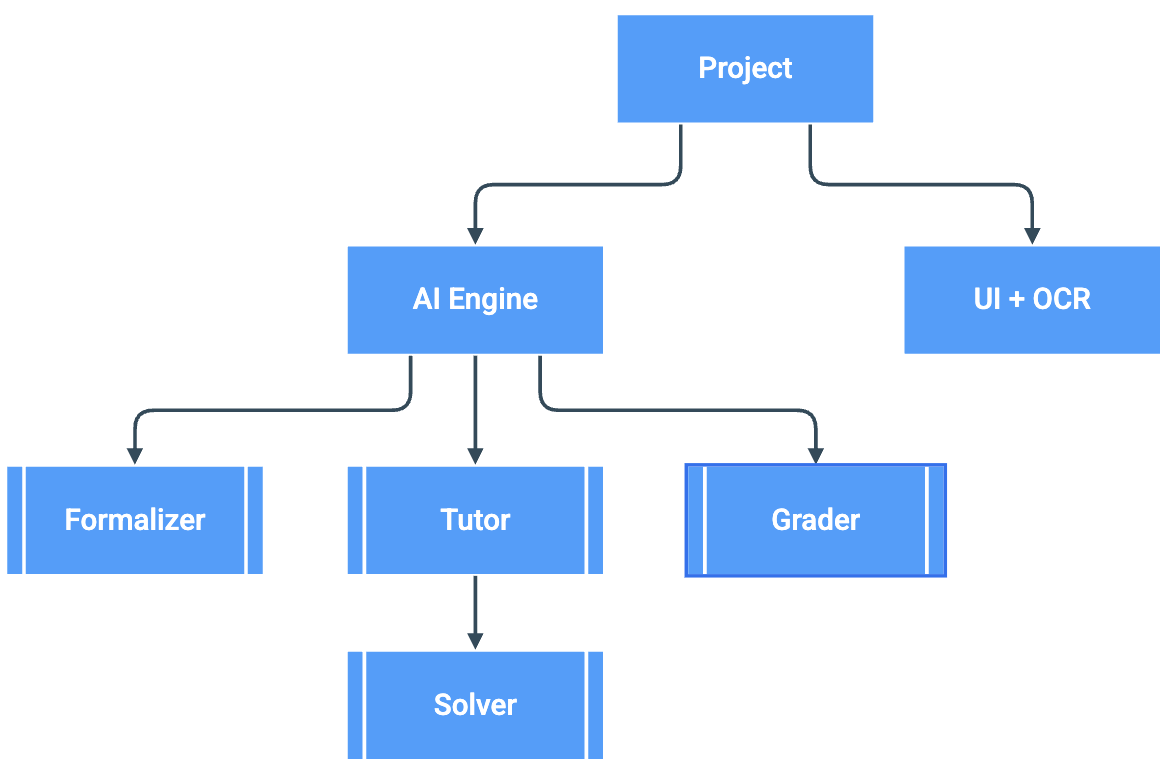
\includegraphics[width=0.9\linewidth]{structure.png}
    \caption{Tổng quan các thành phần của dự án}
    \label{fig:project-overview}
\end{figure}

Khối \textit{UI + OCR} đóng vai trò tiếp nhận dữ liệu từ người dùng.Học sinh có thể cung cấp ảnh chụp đề bài hoặc bài làm thay
vì phải nhập lại toàn bộ nội dung. Thành phần OCR chuyển dữ liệu ảnh thành văn
bản để khối AI tiếp tục phân tích.

\textit{AI Engine} là phần lõi của hệ thống, đảm nhiệm việc xử lý đề bài, lời giải tham chiếu và bài làm của học sinh dưới dạng có cấu trúc. Thay vì để mô hình ngôn ngữ trực tiếp đưa ra kết luận đúng sai, hệ thống chia quá trình xử lý thành các bước rõ ràng: formalize dữ liệu đầu vào, sinh hoặc tiếp nhận lời giải chuẩn, ánh xạ lời giải của học sinh với lời giải chuẩn và chẩn đoán lỗi sai.

Bên trong \textit{AI Engine}, dự án được tổ chức thành ba nhóm chức năng chính. Nhóm \textit{Formalizer} chuyển đề bài, bài mẫu của giáo viên và bài làm của học sinh từ ngôn ngữ tự nhiên sang các thực thể, biểu thức và bước lập luận có cấu trúc. Nhóm \textit{Solver} được sử dụng trong trường hợp chưa có bài mẫu, có nhiệm vụ tạo lời giải tham chiếu từ đề bài và kiểm tra tính hợp lệ của các bước tính toán. Nhóm \textit{Grader} thực hiện ánh xạ giữa lời giải học sinh với bài mẫu hoặc lời giải tham chiếu, từ đó xác định vị trí sai lệch và phân loại nguyên nhân lỗi.

Dự án sử dụng cách tiếp cận hybrid giữa mô hình ngôn ngữ lớn (Large Language Model -- LLM) và xử lý ký hiệu bằng Python. LLM được dùng để hỗ trợ đọc hiểu các cách diễn đạt đa dạng trong đề bài và lời giải, trong khi các bước kiểm tra quan trọng như thực thi biểu thức, kiểm tra đơn vị, ánh xạ thực thể và truy vết lỗi được thực hiện trên biểu diễn có cấu trúc. Cách kết hợp này giúp hệ thống tận dụng khả năng xử lý ngôn ngữ của LLM nhưng vẫn giảm phụ thuộc vào các nhận định tự do dễ gây ảo giác.

Trong phạm vi mã nguồn hiện tại, dự án tập trung triển khai phần lõi của \textit{AI Engine}, bao gồm formalize dữ liệu, sinh lời giải tham chiếu, kiểm tra lời giải và chẩn đoán lỗi trong bài làm của học sinh. Khối \textit{UI + OCR} và cơ chế tạo phản hồi mang tính sư phạm sẽ được phát triển ở các giai đoạn tiếp theo, nhằm giúp hệ thống tiếp nhận bài làm thực tế và đưa ra gợi ý phù hợp hơn cho học sinh.


% =========================================================
% SECTION 2: KIẾN TRÚC HỆ THỐNG
% =========================================================
\section{Kiến trúc hệ thống}

\subsection{Kiến trúc tổng thể}

Luồng hoạt động chi tiết của hệ thống được trình bày trong Hình~\ref{fig:detailed-system-flow}. Hệ thống được tổ chức xung quanh phần lõi \textit{AI Engine}, trong đó các bước xử lý chính gồm formalize dữ liệu đầu vào, sinh lời giải tham chiếu khi cần thiết và so sánh lời giải để chẩn đoán lỗi.

Cụ thể, hệ thống có hai nhánh xử lý chính. Nhánh \textit{Grader} được sử dụng khi đã có bài mẫu hoặc lời giải chuẩn do giáo viên cung cấp. Khi đó, hệ thống formalize đề bài, bài mẫu và bài làm của học sinh, sau đó ánh xạ các bước tương ứng để phát hiện sai lệch trong quá trình lập luận. Nhánh \textit{Solver} được sử dụng trong trường hợp chưa có bài mẫu; hệ thống sẽ sinh lời giải tham chiếu từ đề bài, kiểm tra tính hợp lệ của lời giải này, rồi dùng nó làm cơ sở cho quá trình so sánh và phản hồi.

Cách tổ chức này cho phép hệ thống hoạt động trong cả hai bối cảnh: hỗ trợ giáo viên chấm bài dựa trên lời giải mẫu có sẵn, và hỗ trợ học sinh theo vai trò gia sư khi cần tự sinh lời giải tham chiếu. Các phản hồi hoặc gợi ý cho học sinh được xây dựng dựa trên kết quả chẩn đoán lỗi, thay vì chỉ dựa trên đáp án cuối cùng.


\begin{figure}[htbp]
    \centering
    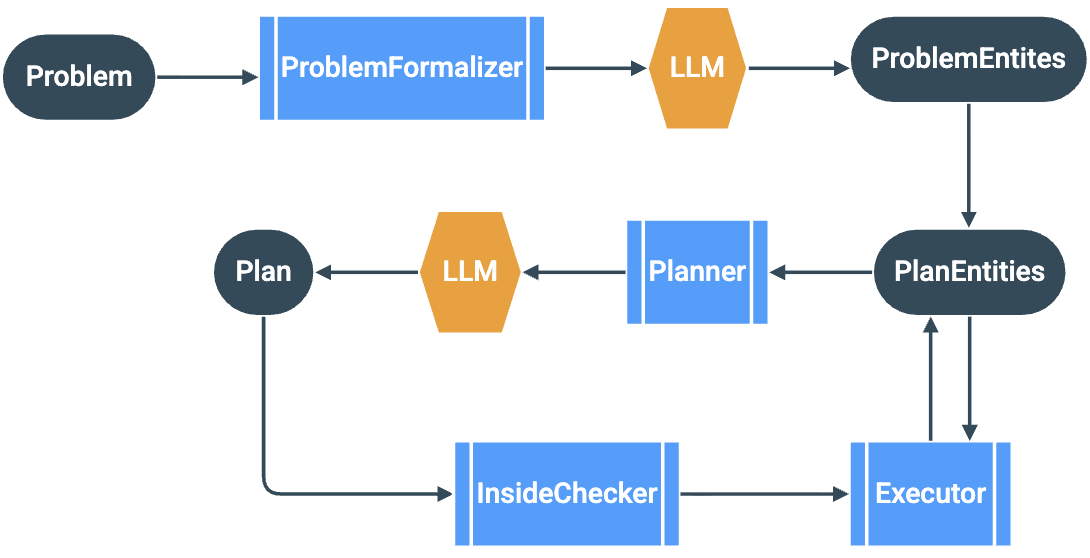
\includegraphics[width=\linewidth]{Solver.png}
    \caption{Luồng hoạt động chi tiết của hệ thống giải toán}
    \label{fig:detailed-system-flow}
\end{figure}

\begin{figure}[htbp]
    \centering
    \includegraphics[width=\linewidth]{Grader.png}
    \caption{Luồng hoạt động chi tiết của hệ thống chấm điểm}
    \label{fig:detailed-system-flow}
\end{figure}

Ở giai đoạn hiện tại, đầu vào của hệ thống là văn bản được nhập trực tiếp.
Trong kiến trúc hoàn chỉnh, nội dung này cũng có thể được trích xuất từ ảnh
chụp thông qua OCR. Sau khi tiếp nhận dữ liệu, hệ thống tạo một lời giải tham
chiếu, phân tích cách làm của học sinh và lần lượt kiểm tra các bằng chứng thu
được. Kết quả cuối cùng không dừng lại ở việc xác định đúng hoặc sai, mà còn
phải đủ rõ để làm cơ sở cho một gợi ý có ích đối với người học.


\subsection{Khối chuẩn hóa và giải bài toán}

\subsubsection{Chuẩn hóa đề bài}

Trước khi thực hiện giải hoặc chấm bài, hệ thống cần chuyển đề bài từ ngôn ngữ tự nhiên sang danh sách các thực thể có cấu trúc. Mỗi thực thể biểu diễn một đại lượng quan trọng trong bài toán, bao gồm giá trị, đơn vị, vị trí xuất hiện, đơn vị tổng quát và phần văn bản gốc tương ứng trong đề bài.

Ví dụ, xét bài toán sau:

\begin{quote}
Ryan started with 36 tokens at the arcade. He used a third of his tokens on Pac-Man, a fourth of his tokens on Candy Crush, and 7 on Ski-ball. Then his parents gave him seven times as many tokens as he spent on Ski-ball. How many tokens did Ryan end up with?
\end{quote}

Sau bước chuẩn hóa, hệ thống chưa sinh lời giải mà chỉ ghi nhận các dữ kiện được cho trực tiếp trong đề bài và đại lượng cần tìm. Kết quả chuẩn hóa có thể được biểu diễn như Bảng~\ref{tab:problem-entities-example}.

\begin{table}[ht]
\centering
\caption{Ví dụ danh sách thực thể được trích xuất từ đề bài}
\label{tab:problem-entities-example}
\small
\begin{tabular}{|p{3.2cm}|p{1.1cm}|p{1.3cm}|p{1.5cm}|p{1.5cm}|p{4.8cm}|}
\hline
\textbf{Tên thực thể} & \textbf{value} & \textbf{unit} & \textbf{location} & \textbf{grand\_unit} & \textbf{source} \\
\hline
\texttt{tokens\_start} & 36 & tokens & input & tokens & Ryan started with 36 tokens at the arcade \\
\hline
\texttt{tokens\_wasted\_pac\_man} & 0.3333 & null & input & null & a third of his tokens on Pac-Man \\
\hline
\texttt{tokens\_wasted\_candy\_crush} & 0.25 & null & input & null & a fourth of his tokens on Candy Crush \\
\hline
\texttt{tokens\_wasted\_ski\_ball} & 7 & tokens & input & tokens & 7 on Ski-ball \\
\hline
\texttt{tokens\_parent\_multiplier} & 7 & null & input & null & seven times as many tokens as he spent on Ski-ball \\
\hline
\texttt{tokens\_end} & null & tokens & target & tokens & How many tokens did Ryan end up with? \\
\hline
\end{tabular}
\end{table}

Trong bảng trên, các thực thể có \textit{location} là \textit{input} tương ứng với những dữ kiện xuất hiện trực tiếp trong đề bài. Chẳng hạn, \texttt{tokens\_start} biểu diễn số token ban đầu của Ryan, \texttt{tokens\_wasted\_ski\_ball} biểu diễn số token dùng cho trò Ski-ball, còn \texttt{tokens\_parent\_multiplier} biểu diễn hệ số ``gấp bảy lần'' được nhắc tới trong đề. Thực thể \texttt{tokens\_end} có \textit{location} là \textit{target}, biểu diễn đại lượng mà bài toán yêu cầu tìm. Vì đại lượng này chưa được tính ở bước chuẩn hóa nên trường \textit{value} được đặt là \textit{null}.

Điểm quan trọng của bước chuẩn hóa là hệ thống không tự thực hiện trước các phép tính trung gian. Ví dụ, hệ thống ghi nhận $\frac{1}{3}$ và $\frac{1}{4}$ như các tỷ lệ được cho trong đề, nhưng chưa tính số token Ryan dùng cho Pac-Man hoặc Candy Crush. Tương tự, hệ thống ghi nhận số token dùng cho Ski-ball là 7 và hệ số cha mẹ cho thêm là 7, nhưng chưa tính ngay $7 \times 7$. Các kết quả trung gian này chỉ được tạo ra ở giai đoạn lập kế hoạch giải và thực thi biểu thức.

Cách biểu diễn này giúp hệ thống phân biệt rõ dữ kiện ban đầu, đại lượng cần tìm và các kết quả được sinh ra thông qua suy luận. Nhờ đó, nhánh sinh lời giải có thể xây dựng các bước tính toán trên nền dữ kiện đã được kiểm soát, còn nhánh chấm bài có thể đối chiếu bài làm của học sinh với lời giải chuẩn một cách rõ ràng hơn.





\subsubsection{Xây dựng lời giải tham chiếu}

Sau bước chuẩn hóa, hệ thống cần xây dựng một lời giải tham chiếu để làm cơ sở
đánh giá bài làm của học sinh. Lời giải này không chỉ chứa đáp án cuối cùng mà
còn thể hiện các bước suy luận cần thiết để đi từ dữ kiện ban đầu đến đại lượng
cần tìm.

Trong phiên bản cải tiến, LLM không trực tiếp viết lời giải cuối cùng. Thay vào
đó, mô hình chỉ chuyển đề bài thành một bản kế hoạch giải có cấu trúc: đâu là dữ
kiện ban đầu, cần thực hiện những phép tính nào, các bước phụ thuộc vào nhau ra
sao, đơn vị của từng đại lượng là gì và câu hỏi cuối cùng yêu cầu tìm đại lượng
nào. Có thể xem đây là bản nháp máy đọc được của lời giải, nhưng chưa phải là
một lời giải hoàn chỉnh để đem đi chấm ngay.

Sau đó, bộ giải của hệ thống thực hiện các phép tính trong bản kế hoạch này. Các
giá trị trung gian không được lấy trực tiếp từ LLM mà phải được tạo ra qua từng
bước tính rõ ràng. Bộ giải xử lý các dạng phép toán thường gặp trong GSM8K như
cộng, trừ, nhân, chia, phần trăm, đổi đơn vị, làm tròn, so sánh hai đại lượng và
một số trường hợp cần suy luận ngược từ kết quả đã biết.

Cách phân chia này giúp hệ thống tận dụng khả năng hiểu ngôn ngữ tự nhiên của
LLM nhưng vẫn kiểm soát được phần tính toán. LLM giúp đọc đề và lập kế hoạch;
bộ giải chịu trách nhiệm tính đúng, giữ lại các bước trung gian và tạo lời giải
tham chiếu để dùng cho khối chẩn đoán lỗi.

\subsubsection{Kiểm tra và đánh giá lời giải tham chiếu}

Lời giải do hệ thống tạo ra chưa được sử dụng ngay để đánh giá bài làm của học
sinh. Trước hết, hệ thống rà soát lại các bước suy luận: phép tính, đơn vị, dữ
kiện được sử dụng và đại lượng trả lời ở bước cuối.

Nếu phát hiện vấn đề, hệ thống gửi thông tin lỗi cho LLM để điều chỉnh kế hoạch
giải, sau đó thực hiện và rà soát lại. Quá trình này giúp hạn chế việc sử dụng
một lời giải tham chiếu chưa hợp lý để đánh giá bài làm của học sinh.

Khi chạy benchmark trên GSM8K, đáp án cuối cùng còn được đối chiếu với đáp án
chính thức để đo độ chính xác của bộ giải. Đáp án này chỉ dùng cho đánh giá thực
nghiệm, không được cung cấp cho hệ thống khi giải bài.

\subsection{Phân tích bài làm của học sinh}

Bài làm của học sinh được chuyển thành một chuỗi bước tính toán theo đúng thứ
tự trình bày. Khác với lời giải tham chiếu, quá trình này không nhằm sửa lại bài
làm. Những phép tính học sinh thực sự viết vẫn được giữ nguyên, kể cả khi kết
quả chưa chính xác hoặc dữ kiện đã bị đọc nhầm.

Việc bảo toàn cách làm ban đầu giúp hệ thống nhận ra nguyên nhân của lỗi. Chẳng
hạn, nếu học sinh sử dụng sai một con số từ đề bài, đây là lỗi đọc đề; nếu sử
dụng đúng dữ kiện nhưng thực hiện phép tính sai, đây là lỗi tính toán. Hai
trường hợp này cần được phân biệt vì cách hỗ trợ học sinh cũng khác nhau.

Trước khi đối chiếu, các đại lượng trong bài làm của học sinh được liên kết với
những đại lượng tương ứng trong lời giải tham chiếu. Việc liên kết dựa trên ý
nghĩa của phép tính thay vì chỉ dựa trên cách đặt tên hoặc số dòng trình bày.
Nhờ đó, hệ thống vẫn nhận ra một lời giải hợp lý khi học sinh gộp bước, tách
bước hoặc thay đổi thứ tự của một số phép tính.

\subsection{Đối chiếu và chẩn đoán lỗi}

Sau khi bài làm của học sinh được chuẩn hóa, hệ thống chuyển sang khối
\textit{Evidence Gate} (\textit{EviGate}) để đối chiếu và chẩn đoán lỗi.
\textit{EviGate} được tổ chức thành ba mức. Hai mức đầu sử dụng các quy tắc và
chương trình logic để xử lý những trường hợp có thể xác định rõ ràng. Mức cuối
chỉ gọi LLM khi các bước trước chưa đủ để đưa ra kết luận.

\subsubsection{EviGate 1: kiểm tra cơ bản}

Mức đầu tiên nhận diện các đặc điểm có thể xác định trực tiếp từ bài làm của
học sinh:

\begin{itemize}[leftmargin=*]
    \item \textbf{Đúng hoàn toàn:} bài làm khớp với lời giải tham chiếu.
    \item \textbf{Trả lời bằng chữ:} một phần hoặc toàn bộ số trong bài làm được
    viết bằng từ ngữ thay vì chữ số.
    \item \textbf{Lỗi chính tả:} tên chủ thể hoặc nội dung trình bày có lỗi chính
    tả.
    \item \textbf{Chỉ trả lời đáp án:} học sinh chỉ đưa ra kết quả cuối cùng mà
    không trình bày quá trình giải.
    \item \textbf{Thiếu đơn vị:} một hoặc nhiều bước trong lời giải không ghi
    đơn vị cần thiết.
    \item \textbf{Sai mục tiêu:} bài làm tính ra một đại lượng khác với yêu cầu
    của đề bài.
\end{itemize}

\subsubsection{EviGate 2: kiểm tra bằng logic}

Mức thứ hai phân tích quan hệ giữa các bước trong bài làm và so sánh với lời
giải tham chiếu. Mục tiêu là nhận diện những khác biệt cần kiểm tra bằng phép
tính và quy tắc logic:

\begin{itemize}[leftmargin=*]
    \item \textbf{Gộp bước:} học sinh kết hợp nhiều bước của lời giải tham chiếu
    thành một bước.
    \item \textbf{Đảo bước:} học sinh thay đổi thứ tự của các bước tương đương
    mà không làm sai lời giải.
    \item \textbf{Tách bước:} học sinh chia một bước thành nhiều bước nhỏ hơn.
    \item \textbf{Tính toán sai:} học sinh lựa chọn đúng phép tính nhưng thực
    hiện phép tính chưa chính xác.
    \item \textbf{Không đổi đơn vị:} học sinh sử dụng trực tiếp các giá trị có
    đơn vị khác nhau mà chưa thực hiện phép đổi cần thiết.
    \item \textbf{Đổi đơn vị sai:} học sinh có thực hiện đổi đơn vị nhưng sử
    dụng sai hệ số hoặc sai chiều chuyển đổi.
\end{itemize}

\subsubsection{EviGate 3: đánh giá bằng LLM}

Một số trường hợp không thể kết luận đầy đủ bằng các quy tắc cố định. Khi đó,
hệ thống mới gọi LLM để xem xét nội dung bài làm:

\begin{itemize}[leftmargin=*]
    \item \textbf{Cách tính khác:} học sinh sử dụng một hướng giải khác với lời
    giải tham chiếu và cần xác định cách làm đó có hợp lý hay không.
    \item \textbf{Lỗi diễn đạt:} câu trả lời tối nghĩa hoặc trình bày không đủ rõ
    để các bước chuẩn hóa hoạt động chính xác.
    \item \textbf{Kiến thức chưa học:} lời giải sử dụng kiến thức vượt quá phạm
    vi chương trình học đang xét.
\end{itemize}

Việc chỉ sử dụng LLM ở mức cuối giúp hệ thống ưu tiên những kết luận có thể kiểm
tra bằng chương trình, đồng thời vẫn xử lý được các trường hợp cần hiểu sâu hơn
về ngữ nghĩa và cách lập luận.

\subsubsection{Kết quả chẩn đoán}

Đầu ra của khối \textit{EviGate} cho biết bài làm có sai hay không, những dạng
lỗi được phát hiện và vị trí xuất hiện của từng lỗi. Kết quả này là cơ sở để hệ
thống lựa chọn gợi ý phù hợp cho học sinh.

\subsection{Tạo gợi ý hỗ trợ học sinh}

Sau khi \textit{EviGate} xác định bài làm có sai hay không, lỗi thuộc loại nào
và xuất hiện ở bước nào, hệ thống có đủ cơ sở để tạo gợi ý cho học sinh. Gợi ý
không nên chỉ lặp lại nhãn lỗi, mà cần chuyển kết quả chẩn đoán thành một phản
hồi mà học sinh có thể dùng để tự sửa bài.

Với mỗi nhóm lỗi, cách gợi ý cần khác nhau. Nếu học sinh tính toán sai, hệ thống
có thể yêu cầu kiểm tra lại phép tính ở bước tương ứng. Nếu học sinh thiếu đơn
vị hoặc không đổi đơn vị, gợi ý nên nhắc lại đại lượng đang được so sánh và đơn
vị cần thống nhất. Nếu học sinh sai mục tiêu, phản hồi nên hướng học sinh quay
lại câu hỏi cuối của đề bài. Với các trường hợp dùng cách tính khác, hệ thống
cần thận trọng hơn: nếu cách làm vẫn hợp lý thì không nên ép học sinh đi theo
đúng lời giải tham chiếu.

Khối \textit{Pedagogy + Hint} được định hướng để thực hiện phần phản hồi này.
Mục tiêu của khối không phải là đưa ngay toàn bộ lời giải, mà là chọn mức hỗ trợ
vừa đủ. Một gợi ý tốt cần giúp học sinh nhìn ra điểm cần sửa nhưng vẫn giữ lại
cơ hội để các em tự hoàn thiện lời giải.

\subsection{Nguồn lời giải tham chiếu}

Trong luồng gia sư chính, lời giải tham chiếu là lời giải do hệ thống tự sinh ở
giai đoạn đầu. Sau khi đề bài được chuẩn hóa thành các đại lượng quan trọng, LLM
được dùng để lập một kế hoạch giải có cấu trúc. Phần còn lại của hệ thống kiểm
tra kế hoạch đó, liên kết các phép tính với dữ kiện đã chuẩn hóa, thực hiện tính
toán và rà soát lại kết quả. Chỉ sau bước này, lời giải mới được dùng làm tham
chiếu để đối chiếu với bài làm của học sinh. Đáp án chính thức trong benchmark
chỉ được dùng ở bước đánh giá cuối cùng, không được đưa vào quá trình sinh lời
giải tham chiếu.

Ngoài nguồn tham chiếu tự sinh, hệ thống cũng hỗ trợ trường hợp đã có sẵn một
lời giải mẫu. Lời giải mẫu này không phải do hệ thống tạo ra ở bước đầu, mà được
cung cấp từ bên ngoài, chẳng hạn lời giải chính thức trong bộ dữ liệu hoặc lời
giải do giáo viên chuẩn bị. Khi đó, hệ thống chuẩn hóa lời giải mẫu thành các
bước tính toán rồi dùng nó làm cơ sở so sánh với bài làm của học sinh.

Hai cách dùng này tương ứng với hai bối cảnh khác nhau. Lời giải tham chiếu tự
sinh phù hợp với vai trò gia sư tự động, khi người dùng chỉ đưa vào đề bài và bài
làm học sinh. Lời giải mẫu có sẵn phù hợp khi muốn chấm theo một đáp án đã được
kiểm soát trước, hoặc khi cần đánh giá riêng khả năng phát hiện lỗi mà không để
chất lượng của bộ tự giải ảnh hưởng đến kết quả.

% =========================================================
% SECTION 3: CHI TIẾT KỸ THUẬT
% =========================================================
\section{Chi tiết kỹ thuật}

\subsection{Biểu diễn dữ liệu trung gian}

Để có thể kiểm tra từng bước giải, hệ thống không làm việc trực tiếp trên văn
bản tự nhiên sau khi đã đọc đầu vào. Thay vào đó, đề bài, lời giải tham chiếu và
bài làm học sinh được chuyển thành các bản ghi có cấu trúc.

\subsubsection{Thực thể}

Mỗi đại lượng trong đề bài được biểu diễn bằng một thực thể. Một thực thể lưu
giá trị, đơn vị, vai trò trong bài toán và bằng chứng trong đề bài. Ví dụ:

\begin{verbatim}
notebooks:
  value: 30
  unit: notebooks
  location: input
  grand_unit: items
  source: there are 30 notebooks on the shelf
\end{verbatim}

Trong đó, \texttt{value} là giá trị số, \texttt{unit} là đơn vị trực tiếp,
\texttt{location} cho biết đại lượng là dữ kiện đầu vào, kết quả trung gian hay
mục tiêu cần tìm, \texttt{grand\_unit} giúp so sánh các đại lượng cùng nhóm, còn
\texttt{source} lưu cụm từ trong đề bài làm bằng chứng cho thực thể đó. Với đại
lượng cần tìm, giá trị ban đầu được để trống và chỉ được điền sau khi hệ thống
thực hiện các bước giải.

Sau khi lời giải được thực hiện, các thực thể trung gian có thêm biểu thức tạo
ra chúng. Chẳng hạn, nếu số bút được tính từ số vở và số bút nhiều hơn số vở,
thực thể kết quả sẽ lưu quan hệ tương ứng. Hệ thống cũng tạo biểu thức mở rộng
để thay các kết quả trung gian bằng dữ kiện ban đầu. Biểu thức mở rộng này giúp
việc so sánh hai cách giải trở nên ổn định hơn.

\subsubsection{Kế hoạch giải}

Lời giải được biểu diễn thành các bước liên tiếp. Mỗi bước chỉ rõ biểu thức cần
tính, tên đại lượng kết quả và đơn vị của kết quả:

\begin{verbatim}
step1:
  expr: notebooks + pens_more_than_notebooks
  result: pens
  result_unit: pens
  result_grand_unit: items

step2:
  expr: notebooks + pens
  result: total_items
  result_unit: items
  result_grand_unit: items
\end{verbatim}

Sau khi thực thi, mỗi bước có thêm phép tính số học cụ thể, ví dụ:

\begin{verbatim}
reported_expr: 30 + 80 = 110
\end{verbatim}

Sự tách biệt giữa \texttt{expr} và \texttt{reported\_expr} rất quan trọng.
\texttt{expr} mô tả quan hệ toán học bằng tên đại lượng, còn
\texttt{reported\_expr} cho biết phép tính số cụ thể đã được thực hiện hoặc học
sinh đã trình bày. Nhờ đó, hệ thống có thể phân biệt lỗi quan hệ với lỗi tính
toán.

\subsection{Các khối xử lý chính}

\subsubsection{Chuẩn hóa đề bài}

Khối chuẩn hóa đề bài dùng LLM để hiểu ngôn ngữ tự nhiên, sau đó dùng các quy
tắc kiểm tra để giữ lại đúng dữ kiện ban đầu. Khối này không được phép đưa vào
những kết quả chỉ có thể có sau khi giải bài toán. Ví dụ, nếu đề bài cho biết có
30 quyển vở và số bút nhiều hơn số vở 50 chiếc, thì 30 và 50 là dữ kiện ban đầu;
số bút thực tế phải được tính ở bước giải sau đó.

Khối này cũng xử lý các dạng dữ kiện thường gặp trong GSM8K như phân số, phần
trăm, số viết bằng chữ, hệ số nhân và đổi đơn vị. Một số hằng số hỗ trợ có thể
được thêm để quá trình giải vẫn biểu diễn bằng biến thay vì viết trực tiếp các
con số rời rạc trong công thức.

\subsubsection{Sinh và thực thi lời giải tham chiếu}

Trong phạm vi mục này, trọng tâm là cách hệ thống tự sinh lời giải tham chiếu từ
đề bài. Đây là phần thứ nhất trong cách chia của dự án: tự giải bài toán để tạo
một lời giải chuẩn. Phần đối chiếu với lời giải mẫu hoặc lời giải của giáo viên
được xem là tầng xử lý sau.

Kỹ thuật chính của phần lời giải tham chiếu là tách việc hiểu đề khỏi việc tính
toán. LLM được dùng ở vai trò đọc ngôn ngữ tự nhiên và lập kế hoạch giải. Bộ
giải của hệ thống mới là thành phần thực hiện phép tính, tạo giá trị trung gian
và đưa ra đáp án cuối cùng. Nhờ cách tách này, hệ thống không để LLM tự trả lời
theo văn bản tự do, mà buộc lời giải phải đi qua các bước có cấu trúc.

Kế hoạch giải có cấu trúc gồm ba nhóm thông tin chính:

\begin{itemize}[leftmargin=*]
    \item \textbf{Dữ kiện ban đầu:} các số liệu xuất hiện trong đề bài, đơn vị
    của chúng và ngữ cảnh đi kèm. Những giá trị chỉ có thể biết sau khi tính toán
    không được đưa vào nhóm này.
    \item \textbf{Các bước tính:} mỗi bước chỉ rõ phép toán cần làm, những đại
    lượng được dùng làm đầu vào, đơn vị của kết quả và ý nghĩa ngắn gọn của bước
    đó.
    \item \textbf{Đại lượng cần tìm:} hệ thống xác định câu hỏi cuối đang hỏi
    đại lượng nào, tránh trường hợp tính đúng một số nhưng trả lời nhầm mục tiêu.
\end{itemize}

Sau khi có kế hoạch, bộ giải thực thi các bước theo quan hệ phụ thuộc giữa các
đại lượng. Một bước chỉ được tính khi các đầu vào của nó đã có giá trị. Nếu một
bước dùng kết quả của bước khác, bộ giải tự lần theo chuỗi phụ thuộc đó để tính
trước giá trị cần thiết. Cách làm này giúp thứ tự trình bày trong kế hoạch không
cần hoàn toàn trùng với thứ tự thực thi, miễn là các quan hệ giữa các bước được
ghi đúng.

Bộ giải không chỉ thực hiện bốn phép tính cơ bản. Để bao phủ các bài toán dạng
GSM8K, hệ thống còn xử lý các nhóm quan hệ thường gặp:

\begin{itemize}[leftmargin=*]
    \item phần trăm, giảm giá, tăng thêm theo phần trăm;
    \item phân số và các cách diễn đạt như một nửa, một phần ba, gấp đôi, gấp ba;
    \item đổi đơn vị và làm tròn khi đề bài yêu cầu số nguyên;
    \item bài toán tỉ lệ, chia tổng theo tỉ lệ hoặc tìm một phần khi biết tổng;
    \item suy luận ngược, chẳng hạn biết số tiền còn lại hoặc tổng sau cùng rồi
    lần ngược để tìm giá trị ban đầu;
    \item các quan hệ so sánh như nhiều hơn, ít hơn, kém hơn một lượng, hoặc
    nhiều hơn theo hệ số nhân.
\end{itemize}

Mỗi bước sau khi được tính sẽ tạo ra một bản ghi gồm biểu thức, tên đại lượng,
giá trị và đơn vị. Vì vậy, đầu ra của bộ giải không chỉ là một con số cuối cùng.
Nó còn là một chuỗi lời giải tham chiếu có thể đọc lại, kiểm tra lại và dùng để
đối chiếu với bài làm của học sinh ở các bước sau.

Đây là lý do bộ giải có thể đạt độ chính xác cao trên benchmark. Phần ngôn ngữ
khó được giao cho LLM xử lý, còn phần số học được thực hiện bằng các quy tắc xác
định. Khi LLM chỉ cần lập kế hoạch thay vì tự tính đáp án, lỗi tính toán ngẫu
nhiên giảm đi đáng kể. Đồng thời, vì mỗi giá trị trung gian đều phải xuất phát
từ dữ kiện ban đầu hoặc từ một bước tính trước đó, hệ thống có thể hạn chế việc
tạo ra những con số không có căn cứ trong đề bài.

\subsubsection{Chuẩn hóa bài làm học sinh và lời giải mẫu}

Bài làm học sinh được chuẩn hóa theo cùng kiểu biểu diễn bước giải, nhưng có một
nguyên tắc khác với lời giải tham chiếu: hệ thống phải giữ đúng phép tính học
sinh đã viết. Nếu học sinh viết một phép tính sai, phép tính đó không được tự
động sửa trong bước chuẩn hóa, vì chính nó là bằng chứng để phát hiện lỗi.

Khi có sẵn lời giải mẫu, hệ thống cũng chuẩn hóa lời giải đó thành các bước tính
toán. Lời giải mẫu có thể đến từ đáp án chính thức trong dữ liệu hoặc từ giáo
viên. Nó được dùng như một nguồn tham chiếu thay thế cho lời giải tự sinh khi
cần chấm theo một cách giải đã được kiểm soát trước.

\subsubsection{Ánh xạ và so sánh hai lời giải}

Hai lời giải có thể sử dụng tên đại lượng khác nhau hoặc chia bước khác nhau.
Vì vậy, trước khi kết luận đúng sai, hệ thống cần ánh xạ đại lượng trong bài làm
học sinh với đại lượng tương ứng trong lời giải tham chiếu. Việc ánh xạ dựa
trên dữ kiện chung, tên kết quả, biểu thức tạo ra đại lượng và biểu thức mở
rộng về dữ kiện ban đầu.

Trong quá trình so sánh, hệ thống không yêu cầu hai lời giải giống hệt nhau về
hình thức. Các phép cộng và phép nhân có thể đổi thứ tự toán hạng; học sinh cũng
có thể gộp hoặc tách bước mà vẫn giữ đúng quan hệ toán học. Điều hệ thống cần
xác định là cách lập luận đó có dẫn đến đúng đại lượng cần tìm hay không.

\subsection{Cơ chế phát hiện lỗi}

Cơ chế phát hiện lỗi gồm ba nhóm kiểm tra. Nhóm thứ nhất rà soát một lời giải
riêng lẻ, chẳng hạn phép tính có đúng không, đơn vị có bị thiếu không, có dùng
kết quả chưa được tạo ra không hoặc có tính nhầm đại lượng mục tiêu không. Nhóm
thứ hai so sánh bài làm học sinh với lời giải tham chiếu để phát hiện sai quan
hệ, đổi đơn vị sai, gộp bước, tách bước, đảo bước hoặc cách tính khác. Nhóm thứ
ba dùng LLM như một lớp đánh giá bổ sung cho những trường hợp mà quy tắc cố định
khó kết luận.

Kết quả cuối cùng được tổng hợp thành trạng thái đúng sai và danh sách lỗi. Mỗi
lỗi gồm loại lỗi, bước liên quan và đại lượng liên quan nếu xác định được. Cách
tổ chức này giúp hệ thống không chỉ biết bài làm có đúng hay không, mà còn biết
lỗi xuất hiện ở đâu và thuộc loại nào.

% =========================================================
% SECTION 4: BENCHMARK
% =========================================================
\section{Dữ liệu benchmark và phương pháp đánh giá}

\subsection{Mục đích xây dựng benchmark}

Benchmark của dự án được xây dựng để kiểm tra một câu hỏi cụ thể: hệ thống có
thực sự nhận ra lỗi trong quá trình giải của học sinh hay chỉ đang so khớp đáp
án cuối cùng. Vì vậy, mỗi mẫu không chỉ có đề bài và đáp án đúng, mà còn có một
bài làm học sinh được tạo có chủ đích để chứa một hoặc nhiều kiểu sai sót.

Nguồn bài toán dựa trên dạng GSM8K, tức là các bài toán đố nhiều bước, có ngữ
cảnh đời sống và yêu cầu suy luận số học bằng ngôn ngữ tự nhiên. Lời giải sai
được chỉnh sửa thủ công từ lời giải đúng hoặc từ một lời giải gần đúng, sao cho
lỗi vẫn giống lỗi mà học sinh có thể mắc trong thực tế. Cách xây dựng này giúp
benchmark không chỉ đo việc trả lời đúng hay sai, mà còn đo khả năng chỉ ra sai
ở đâu và sai theo kiểu nào.

\subsection{Cấu trúc và cách gán nhãn dữ liệu}

Trong phiên bản CSV hiện có trong thư mục dự án, tập benchmark gồm 300 bài toán.
Trong đó, 200 mẫu đã được gán nhãn thủ công cho bài làm học sinh và 100 mẫu còn
lại chủ yếu được dùng để mở rộng đánh giá khả năng tạo lời giải tham chiếu. Mỗi
dòng dữ liệu gồm đề bài, đáp án đúng, lời giải tham chiếu, bài làm học sinh, nhãn
đúng sai, loại lỗi và vị trí bắt đầu xuất hiện lỗi. Trường \texttt{wrong} cho
biết bài làm có sai về mặt toán học hay không, còn \texttt{type} mô tả dạng lỗi
cụ thể. Một mẫu có thể có nhiều nhãn lỗi, chẳng hạn vừa sai quan hệ vừa gộp
bước. Trường \texttt{wrong location} được dùng để ghi lại bước bắt đầu sai trong
lời giải; ở quy trình đánh giá hiện tại, trường này chủ yếu dùng cho phân tích
thủ công và chưa được tính thành chỉ số riêng.

\begin{table}[H]
    \centering
    \begin{tabular}{p{0.38\linewidth} p{0.22\linewidth} p{0.22\linewidth}}
        \toprule
        \textbf{Trạng thái bài làm} & \textbf{Số mẫu} & \textbf{Tỷ lệ} \\
        \midrule
        Bài làm sai (\texttt{wrong=yes}) & 133 & 66.5\% \\
        Bài làm không sai (\texttt{wrong=no}) & 67 & 33.5\% \\
        \bottomrule
    \end{tabular}
    \caption{Phân bố nhãn đúng sai trên 200 mẫu đã gán nhãn thủ công}
\end{table}



\subsection{Hệ thống nhãn lỗi}

Các nhãn lỗi bao phủ cả lỗi trình bày và lỗi toán học. Những nhãn như gộp bước,
tách bước, đảo bước, trả lời bằng chữ hoặc lỗi chính tả thường không làm bài sai
nếu lập luận vẫn đúng. Ngược lại, các nhãn như tính toán sai, sai quan hệ, đọc
sai đề, sai mục tiêu hoặc đổi đơn vị sai thường ảnh hưởng trực tiếp đến kết quả.

\begin{table}[H]
    \centering
    \small
    \begin{tabular}{p{0.27\linewidth} p{0.39\linewidth} p{0.12\linewidth} p{0.12\linewidth}}
        \toprule
        \textbf{Nhãn} & \textbf{Ý nghĩa chính} & \textbf{Số mẫu} & \textbf{Tỷ lệ} \\
        \midrule
        Sai quan hệ & Dùng sai phép toán, sai công thức hoặc sai quan hệ giữa các đại lượng. & 36 & 18.0\% \\
        Tính toán sai & Quan hệ đúng nhưng phép tính số học bị sai. & 36 & 18.0\% \\
        Cách tính khác & Dùng hướng giải khác lời giải tham chiếu nhưng vẫn hợp lý. & 21 & 10.5\% \\
        Lỗi logic & Suy luận không hợp lệ, khó quy về một lỗi tính toán đơn lẻ. & 20 & 10.0\% \\
        Đọc sai đề & Dùng sai dữ kiện hoặc hiểu sai điều kiện trong đề bài. & 20 & 10.0\% \\
        Gộp bước & Gộp nhiều bước tham chiếu thành một bước. & 18 & 9.0\% \\
        Sai mục tiêu & Tính ra đại lượng khác với đại lượng câu hỏi yêu cầu. & 13 & 6.5\% \\
        Thiếu bước & Bỏ qua bước cần thiết trong lập luận. & 12 & 6.0\% \\
        Bước thừa & Thêm bước không cần thiết hoặc không liên quan trực tiếp. & 11 & 5.5\% \\
        Lỗi diễn đạt & Trình bày tối nghĩa, gây khó khăn cho việc chuẩn hóa thành bước tính. & 11 & 5.5\% \\
        Trả lời bằng chữ & Dùng chữ để biểu diễn một phần hoặc toàn bộ đáp án số. & 11 & 5.5\% \\
        Lỗi chính tả & Sai chính tả ở chủ thể hoặc cách gọi đại lượng. & 11 & 5.5\% \\
        Tách bước & Chia nhỏ một bước tham chiếu thành nhiều bước hợp lệ. & 11 & 5.5\% \\
        Thiếu đơn vị & Không ghi đơn vị ở một hoặc nhiều bước. & 11 & 5.5\% \\
        Đảo bước & Thay đổi thứ tự các bước tương đương. & 10 & 5.0\% \\
        Đổi đơn vị sai & Có đổi đơn vị nhưng dùng sai hệ số hoặc sai chiều đổi. & 8 & 4.0\% \\
        Đúng hoàn toàn & Lời giải khớp với lời giải đúng, dùng để kiểm tra trường hợp không lỗi. & 6 & 3.0\% \\
        Không đổi đơn vị & Bỏ qua bước đổi đơn vị cần thiết. & 5 & 2.5\% \\
        Chỉ trả lời đáp án & Chỉ đưa đáp án cuối, thiếu quá trình lập luận. & 5 & 2.5\% \\
        \bottomrule
    \end{tabular}
    \caption{Thống kê nhãn lỗi trên 200 mẫu đã gán nhãn thủ công. Một mẫu có thể có nhiều nhãn nên tổng tỷ lệ lớn hơn 100\%.}
\end{table}

Hai nhóm lỗi xuất hiện nhiều nhất là sai quan hệ và tính toán sai. Điều này phù
hợp với mục tiêu của dự án, vì đây là hai lỗi mà một hệ thống gia sư cần phân
biệt rõ: học sinh có thể hiểu đúng hướng làm nhưng tính nhầm, hoặc ngược lại,
tính toán đúng trên một quan hệ vốn đã sai.

\subsection{Phương pháp đánh giá}

Phương pháp đánh giá được chia thành hai phần để tránh lẫn lộn giữa khả năng
giải bài và khả năng chấm bài. Trước hết, hệ thống được kiểm tra ở vai trò tạo
lời giải tham chiếu từ đề bài. Với mỗi bài toán, bộ giải đọc đề, chuẩn hóa các
đại lượng, sinh kế hoạch giải và thực thi các bước tính để tìm đại lượng mục
tiêu. Kết quả cuối cùng được so sánh với đáp án chính thức trong benchmark. Phần
này cho biết hệ thống có tạo được một lời giải chuẩn đủ tin cậy để làm nền cho
các bước chẩn đoán phía sau hay không.

Sau đó, hệ thống được đánh giá ở vai trò chấm bài làm học sinh. Ở phần này, mỗi
mẫu benchmark gồm đề bài, lời giải tham chiếu và bài làm học sinh. Hệ thống đưa
cả lời giải tham chiếu và bài làm học sinh về cùng một dạng biểu diễn bước giải,
sau đó so sánh từng quan hệ, từng phép tính và từng đại lượng được tạo ra. Đầu
ra của hệ thống gồm kết luận bài làm sai hay không, loại lỗi được phát hiện và
vị trí lỗi nếu xác định được. Kết quả này được đối chiếu với nhãn thủ công trong
benchmark.

Cách đánh giá này phù hợp với mục tiêu của dự án hơn việc chỉ so đáp án cuối.
Một học sinh có thể ra đáp án đúng nhưng trình bày thiếu bước, dùng cách tính
khác hoặc gộp nhiều bước lại. Ngược lại, có trường hợp đáp án sai nhưng nguyên
nhân sai nằm ở một bước rất sớm, chẳng hạn đọc nhầm dữ kiện hoặc chọn sai quan
hệ giữa hai đại lượng. Vì vậy, hệ thống cần được đánh giá theo cả kết luận đúng
sai và khả năng nhận diện bản chất lỗi.

Ngoài quy trình chính, dự án còn có một hướng so sánh với mô hình ngôn ngữ dùng
trực tiếp trên văn bản. Ở hướng này, mô hình nhận đề bài, lời giải tham chiếu và
bài làm học sinh rồi tự đưa ra nhãn lỗi. Đây là mốc đối chứng để xem phần biểu diễn
có cấu trúc và các bước kiểm tra logic của hệ thống mang lại cải thiện như thế
nào so với việc để LLM chấm trực tiếp.

\subsection{Kết quả đánh giá}

Trong lần đánh giá gần nhất, bộ giải tham chiếu được chạy trên 300 bài toán
GSM8K trong benchmark cục bộ của dự án. Với mỗi bài, hệ thống dùng phần đề bài
để tạo lời giải tham chiếu, lấy đáp án cuối cùng do bộ giải sinh ra và so sánh
với đáp án chính thức. Đáp án chính thức chỉ được dùng cho bước đối chiếu kết
quả, không được cung cấp cho hệ thống trong quá trình giải.

\begin{table}[H]
    \centering
    \begin{tabular}{p{0.4\linewidth} p{0.18\linewidth} p{0.32\linewidth}}
        \toprule
        \textbf{Chỉ số / Phương pháp} & \textbf{Giá trị} & \textbf{Ý nghĩa} \\
        \midrule
        Số mẫu đánh giá & 300 & Toàn bộ bài toán được dùng trong lần chạy này \\
        Số mẫu đúng (Bộ giải tham chiếu) & 291 & Đáp án cuối cùng trùng đáp án chính thức \\
        Số mẫu sai (Bộ giải tham chiếu) & 9 & Bộ giải chạy được nhưng đáp án chưa khớp \\
        Số mẫu lỗi khi chạy & 0 & Không có bài nào bị dừng giữa quá trình giải \\
        \midrule
        \textbf{Độ chính xác Base} & \textbf{48.50\%} & Tỷ lệ đúng khi chạy mô hình nền tảng cơ bản \\
        \textbf{Độ chính xác CoT} & \textbf{94.50\%} & Tỷ lệ đúng khi áp dụng Chain-of-Thought tiêu chuẩn \\
        \textbf{Độ chính xác Bộ giải tham chiếu} & \textbf{97.00\%} & Tỷ lệ đúng tối ưu đạt được của hệ thống \\
        \bottomrule
    \end{tabular}
    \caption{Kết quả đối sánh độ chính xác và hiệu năng của bộ giải tham chiếu trên 300 mẫu GSM8K cục bộ}
\end{table}

Kết quả này cho thấy phần tạo lời giải tham chiếu đã đủ ổn định để làm nền cho
các bước chẩn đoán lỗi phía sau. Hệ thống đạt độ chính xác vượt trội ($97.00\%$), 
thể hiện mức cải thiện rất mạnh mẽ so với cấu hình chạy mô hình Base thông thường 
($48.5\%$) cũng như phương pháp kích hoạt chuỗi suy nghĩ CoT chuẩn ($94.5\%$). 
Sự cải thiện này minh chứng rằng bộ giải không chỉ đơn thuần trả về đáp án 
mà còn sinh ra danh sách bước trung gian có biểu thức, kết quả và đơn vị một cách 
gãy gọn và chính xác. 

Việc không có bài nào bị dừng giữa chừng cũng cho thấy bộ giải đã xử lý được 
toàn bộ các kế hoạch giải trong lần đánh giá này. Những lỗi còn lại chiếm tỷ lệ 
rất nhỏ ($3.00\%$), chủ yếu đến từ việc hệ thống hiểu chưa đúng một số quan hệ 
trong đề bài hoặc chưa có đủ luật xử lý cho các cấu trúc ngôn ngữ khó.



% =========================================================
% SECTION 6: HẠN CHẾ VÀ HƯỚNG PHÁT TRIỂN
% =========================================================
\section{Hạn chế và hướng phát triển}

Mặc dù bộ giải tham chiếu đạt độ chính xác cao khi so đáp án cuối cùng, kết quả
này chưa đồng nghĩa với việc toàn bộ quy trình gia sư đã được đánh giá đầy đủ.
Độ chính xác 97.00\% mới phản ánh khả năng tạo lời giải tham chiếu trên 300 bài
GSM8K cục bộ. Phần chẩn đoán lỗi của học sinh còn cần được đo bằng các chỉ số
riêng, chẳng hạn hệ thống có kết luận đúng bài làm sai hay không, có gọi đúng
loại lỗi hay không và có chỉ đúng vị trí bắt đầu sai hay không.

Một hạn chế khác là chất lượng của hệ thống vẫn phụ thuộc vào bản kế hoạch giải
được tạo ra từ đề bài. Nếu bản kế hoạch này biểu diễn sai quan hệ, ví dụ nhầm
điều kiện thời gian, thiếu bước chia đều hoặc hiểu sai một cụm đếm trong đề bài,
bộ giải có thể tính toán đúng trên một kế hoạch vốn đã sai. Vì vậy, cần bổ sung
bước kiểm tra kế hoạch trước khi giải, chẳng hạn kiểm tra dữ kiện đã dùng, đơn
vị, mối liên hệ giữa câu hỏi cuối và đại lượng cần tìm, cũng như các mẫu ngôn
ngữ dễ gây nhầm lẫn.

Các hướng phát triển trực tiếp từ kết quả benchmark gồm:

\begin{itemize}[leftmargin=*]
    \item xây dựng bộ kiểm thử riêng cho 9 mẫu bộ giải còn sai, để mỗi lần sửa
    luật hoặc cách lập kế hoạch đều có thể kiểm tra lại ngay;
    \item tách riêng ba nhóm đánh giá: chất lượng lập kế hoạch giải, độ chính
    xác của bộ giải và độ chính xác của phần chẩn đoán lỗi học sinh;
    \item chuẩn hóa bản kế hoạch giải chặt hơn, bao gồm kiểm tra kiểu phép toán,
    đơn vị, đại lượng cần tìm, dữ kiện không được dùng và các bước không góp phần
    tạo đáp án;
    \item mở rộng bộ luật cho các bài toán điều kiện, lịch, tuổi, chia tỉ lệ và
    các trường hợp đếm vật thể được mô tả bằng nhiều cụm từ trong cùng một câu;
    \item bổ sung cơ chế báo độ tin cậy của lời giải tham chiếu, để khối chẩn
    đoán lỗi không dùng một lời giải tham chiếu chưa đủ chắc chắn.
\end{itemize}
\section{Tích hợp pipeline vào sản phẩm}

Phần sản phẩm được xây dựng nhằm đưa pipeline vào một quy trình có thể sử dụng
trong thực tế. Giáo viên có thể nhập đề bài, kiểm tra lại nội dung OCR, chỉnh sửa
cấu trúc bài toán và sinh rubric. Rubric sau khi được giáo viên chỉnh sửa được
xem là nguồn chính thức để sử dụng trong quá trình chấm bài.

Đối với bài làm học sinh, hệ thống hỗ trợ tải nhiều tệp, theo dõi tiến trình OCR,
kiểm tra thông tin học sinh, sắp xếp trang và ánh xạ nội dung vào từng bài toán.
Sau khi hoàn tất bước rà soát, bài làm được chuyển tới pipeline chấm điểm. Kết quả
pipeline được đóng gói thành một hợp đồng dữ liệu thống nhất để giao diện hiển thị
điểm, lỗi chẩn đoán và các trường hợp cần giáo viên xem lại.

Để quá trình tích hợp ổn định hơn, mỗi lần sinh rubric và chấm bài được thực thi
trong workspace tạm riêng. Hệ thống cũng ghi log theo từng trace, lưu các đầu vào,
đầu ra trung gian và lỗi theo từng bước. Khi pipeline không trả về kết quả đủ tin
cậy, sản phẩm không tự suy diễn điểm mà đánh dấu bài làm cần được kiểm tra thủ công.

% =========================================================
% SECTION 7: OCR
% =========================================================
\section{Nhận dạng văn bản từ ảnh bằng OCR}



\subsection{Tích hợp OCR với pipeline kiểm tra lời giải}



OCR được sử dụng cho cả đề bài và bài làm học sinh. Mỗi trang tài liệu được lưu
cùng ảnh xem trước, nội dung trích xuất và thông tin nguồn. Trước khi dữ liệu được
đưa vào pipeline, giáo viên có thể sửa văn bản, chọn trang cần sử dụng và xác nhận
thứ tự trang. Nội dung sau khi giáo viên rà soát mới được dùng để phân tách bài toán,
sinh rubric hoặc ánh xạ bài làm học sinh.

Sau bước rà soát, văn bản đề bài được phân tách thành các bài toán và phần nhỏ để
pipeline sinh lời giải tham chiếu cùng rubric. Văn bản bài làm học sinh được ánh xạ
vào các phần tương ứng trước khi chấm. Cách tổ chức này giúp tách riêng lỗi nhận
dạng văn bản với lỗi xử lý của pipeline, đồng thời cho phép giáo viên sửa dữ liệu
đầu vào mà không cần tải lại tài liệu.



% =========================================================
% SECTION 8: KẾT LUẬN
% =========================================================
\section{Kết luận}

Dự án đã xây dựng được lõi của một hệ thống gia sư toán học theo hướng kết hợp
LLM với kiểm tra có cấu trúc. Thay vì để mô hình ngôn ngữ trực tiếp quyết định
đáp án hoặc chấm bài, hệ thống chuyển đề bài và lời giải về các biểu diễn trung
gian có thể thực thi, từ đó tạo lời giải tham chiếu, đối chiếu từng bước và làm
cơ sở cho việc chẩn đoán lỗi.

Phần lời giải tham chiếu là một cải tiến quan trọng của quy trình. Với một bản
kế hoạch giải có cấu trúc và bộ giải theo quy tắc xác định, hệ thống đạt 291/300
mẫu đúng trên benchmark GSM8K cục bộ, tương ứng 97.00\% khi đánh giá theo đáp án
cuối cùng. Kết quả này cho thấy cách tách vai trò giữa LLM và bộ giải là phù hợp:
LLM hỗ trợ hiểu ngôn ngữ tự nhiên, còn bộ giải chịu trách nhiệm tính toán và tạo
chuỗi bước có thể kiểm tra.

Trong các bước tiếp theo, trọng tâm cần chuyển từ việc chỉ tăng độ chính xác đáp
án cuối sang đánh giá đầy đủ khả năng chẩn đoán lỗi học sinh. Khi lời giải tham
chiếu đủ tin cậy, hệ thống có thể tiếp tục hoàn thiện các chỉ số về loại lỗi, vị
trí lỗi và chất lượng gợi ý, đồng thời tích hợp OCR để tiếp nhận bài làm trong
bối cảnh sử dụng thực tế.



\end{document}